\section*{BÀI TẬP CUỐI CHƯƠNG 8}
\subsection{Câu hỏi trắc nghiệm}

\Opensolutionfile{ans}[ans/ans-9C8-OTC]

\begin{ex}%[Dự án EX-9-Đề Cương Toán 9]%[Nguyễn Cường]%[9D6N1-1]
	Tổ $1$ gồm $4$ học sinh là Trung, Hậu, Đảm, Đang. Trong các hoạt động sau, hoạt động nào là phép thử ngẫu nhiên?
	\choice
	{Chọn ra đồng thời $4$ học sinh từ Tổ $1$}
	{Chọn ra học sinh có tên bắt đầu bằng chữ cái T từ Tổ $1$}
	{Chọn ra học sinh có tên bắt đầu bằng chữ cái H từ Tổ $1$}
	{\True Chọn ra học sinh có tên bắt đầu bằng chữ cái Đ từ Tổ $1$}
	\loigiai{
		Hoạt động chọn ra đồng thời $4$ học sinh từ Tổ $1$ chỉ có một kết quả xảy ra nên không là phép thử ngẫu nhiên.\\
		Hoạt động chọn ra học sinh có tên bắt đầu bằng chữ cái T từ Tổ $1$ chỉ có một kết quả xảy ra nên không là phép thử ngẫu nhiên.\\
		Hoạt động chọn ra học sinh có tên bắt đầu bằng chữ cái H từ Tổ $1$ chỉ có một kết quả xảy ra nên không là phép thử ngẫu nhiên.\\
		Hoạt động chọn ra học sinh có tên bắt đầu bằng chữ cái Đ từ Tổ $1$ có hai kết quả có thể xảy ra là chọn bạn Đảm hoặc bạn Đang nên ta không thể biết trước được kết quả của nó. Do đó, đây là một phép thử ngẫu nhiên.
	}
\end{ex}

\begin{ex}%[Dự án EX-9-Đề Cương Toán 9]%[Nguyễn Cường]%[9D6H1-1]
	Một hộp chứa $3$ quả bóng bàn và $2$ quả bóng gôn. Trong các hoạt động sau, hoạt động nào là phép thử ngẫu nhiên?
	\choice
	{Chọn ra đồng thời $5$ quả bóng từ hộp}
	{\True Chọn ra lần lượt $5$ quả bóng từ hộp, bóng lấy ra không được trả lại hộp}
	{Chọn ra đồng thời $2$ quả bóng gôn từ hộp}
	{Chọn ra đồng thời $3$ quả bóng bàn từ hộp}
	\loigiai{
		Hoạt động \lq\lq Chọn ra lần lượt $5$ quả bóng từ hộp, bóng lấy ra không được trả lại hộp\rq\rq\, có nhiều kết quả có thể xảy ra, chẳng hạn $5$ quả bóng lần lượt được lấy ra là: bóng bàn, bóng gôn, bóng bàn, bóng gôn, bóng bàn; bóng bàn, bóng bàn, bóng gôn, bóng bàn, bóng gôn; $\ldots$\\
		Do đó ta không thể biết trước được kết quả của nó, nhưng ta có thể biết tất cả các kết quả có thể xảy ra của nó. Vì vậy, hoạt động này là phép thử ngẫu nhiên.
	}
\end{ex}

\begin{ex}%[Dự án EX-9-Đề Cương Toán 9]%[Nguyễn Cường]%[9D6N1-1]
	Đội bóng bàn lớp 9C gồm $2$ bạn nam là Long và Hoàng, $2$ bạn nữ là Hà và Thanh. Huấn luyện viên chọn ra ngẫu  nhiên một đôi nam nữ từ đội để đi thi đấu. Hãy liệt kê không gian mẫu của phép chọn ngẫu nhiên này.
	\choice
	{\True Long và Hà; Long và Thanh; Hoàng và Hà; Hoàng và Thanh}
	{Long và Thanh; Hoàng và Hà; Hoàng và Thanh}
	{Long và Hà; Long và Thanh; Hoàng và Hà}
	{Long và Hà; Long và Hoàng; Hoàng và Hà; Hoàng và Thanh}
	\loigiai{
	Các cách chọn ngẫu nhiên một đôi nam nữ là: Long và Hà; Long và Thanh; Hoàng và Hà; Hoàng và Thanh.
	}
\end{ex}

\begin{ex}%[Dự án EX-9-Đề Cương Toán 9]%[Nguyễn Cường]%[9D6N1-1]
	Một hộp chứa $3$ tấm thẻ cùng loại được đánh số lần lượt là $6$; $7$; $8$. Bạn Việt lấy lần lượt $3$ tấm thẻ từ hộp một cách ngẫu nhiên. Tấm thẻ lấy ra không được trả lại. Số phần tử của không gian mẫu của phép thử là
	\choice
	{$5$}
	{\True $6$}
	{$7$}
	{$9$}
	\loigiai{
 	Kí hiệu $(x;y;z)$ là kết quả bạn Việt lần lượt lấy được tấm thẻ đánh số $x$, $y$, $z$.\\
 	Không gian mẫu của phép thử là
 	\[\Omega=\{(6;7;8);(6;8;7);(7;6;8);(7;8;6);(8;6;7);(8;7;6)\}.\]
 	Không gian mẫu của phép thử có $6$ phần tử.
	}
\end{ex}

\begin{ex}%[Dự án EX-9-Đề Cương Toán 9]%[Nguyễn Cường]%[9D6N1-1]
	Một hộp chứa $1$ quả bóng màu vàng, $1$ quả bóng màu trắng và $1$ quả bóng màu cam. Các quả bóng có cùng kích thước và khối lượng. Bạn Ánh lấy ra ngẫu nhiên lần lượt $2$ quả bóng từ hộp. Số phần tử của không gian mẫu của phép thử là
	\choice
	{$3$}
	{$4$}
	{$5$}
	{\True$6$}
	\loigiai{
	Kí hiệu $T$ là màu trắng, $V$ là màu vàng và $C$ là màu cam.\\
	Không gian mẫu của phép thử là 
\[\Omega=\{TV;VT;TC;CT;VC;CV\}.\]
Không gian mẫu của phép thử có $6$ phần tử.
	}
\end{ex}

\begin{ex}%[Dự án EX-9-Đề Cương Toán 9]%[Nguyễn Cường]%[9D6H2-2]
	Một hộp chứa $1$ quả bóng màu vàng, $1$ quả bóng màu trắng và $1$ quả bóng màu cam. Các quả bóng có cùng kích thước và khối lượng. Bạn Ánh lấy ra ngẫu nhiên lần lượt $2$ quả bóng từ hộp. Xác suất của biến cố \lq\lq Có $1$ quả bóng màu vàng trong $2$ quả bóng lấy ra\rq\rq~là
	\choice
	{$0$}
	{$\dfrac{1}{3}$}
	{\True$\dfrac{2}{3}$}
	{$\dfrac{1}{2}$}
	\loigiai{
		Kí hiệu $T$ là màu trắng, $V$ là màu vàng và $C$ là màu cam.\\
		Không gian mẫu của phép thử là 
		\[\Omega=\{TV;VT;TC;CT;VC;CV\}.\]
		Không gian mẫu của phép thử có $6$ phần tử nên $n(\Omega)=6$.\\
		Biến cố $A$ \lq\lq Có $1$ quả bóng màu vàng trong $2$ quả bóng lấy ra\rq\rq.\\
		Khi đó, $A=\{TV;VT;VC;CV\}$.\\
		Suy ra $n(A)=2+2=4$.\\
		Xác suất của biến cố $A$ là $\mathrm{P}(A)=\dfrac{n(A)}{n(\Omega)}=\dfrac{4}{6}=\dfrac{2}{3}$.
	}
\end{ex}

\begin{ex}%[Dự án EX-9-Đề Cương Toán 9]%[Nguyễn Cường]%[9D6H2-2]
	Một hộp chứa $3$ viên bi màu vàng lần lượt ghi các số $1$; $2$; $3$ và $2$ viên bi màu xanh lần lượt ghi các số $4$; $5$. Các viên bi có cùng kích thước và khối lượng. Lấy ngẫu nhiên đồng thời hai viên bi trong hộp đó. Xác suất của biến cố $A\colon$ \lq\lq Hai viên bi lấy ra cùng màu\rq\rq.
	\choice
	{$\dfrac{1}{6}$}
	{\True $\dfrac{2}{5}$}	
	{$\dfrac{1}{5}$}	
	{$\dfrac{1}{10}$}	
	\loigiai{
		Không gian mẫu của lấy đồng thời hai viên bi trong hộp là
		\[\Omega=\{ \{1;2\}; \{1;3\}; \{1;4\}; \{1;5\}; \{2;3\}; \{2;4\}; \{2;5\}; \{3;4\}; \{3;5\}; \{4;5\} \}.\]
		Trong đó $\{x;y\}$ là kết quả lấy được viên bi ghi số $x$ và viên bi ghi số $y$.\\
		Suy ra $n(\Omega)=10$.\\
		Các kết quả thuận lợi của biến cố $A$ là $\{1;2\}; \{1;3\}; \{2;3\}; \{4;5\}$.\\
		Do đó, $n(A)=4$.\\
		Xác suất của biến cố $A$ là $\mathrm{P}(A)=\dfrac{n(A)}{n(\Omega)}=\dfrac{4}{10}=\dfrac{2}{5}.$
	}
\end{ex}

\begin{ex}%[Dự án EX-9-Đề Cương Toán 9]%[Nguyễn Cường]%[9D6H2-2]
	Có $3$ phong bì giống nhau lần lượt được đánh số thứ tự từ $1$ đến $3$ và $3$ con tem lần lượt được đánh số thứ tự từ $1$ đến $3$. Dán $3$ con tem đó vào $3$ phong bì sao cho không có phong bì nào không có tem. Tính xác suất của biến cố $A$: \lq\lq Lấy ra được $2$ phong bì trong $3$ phong bì trên sao cho mỗi phong bì đều có số thứ tự giống với số thứ tự con tem đã dán vào nó\rq\rq.
	\choice
	{$\dfrac{1}{3}$}
	{\True$\dfrac{1}{6}$}
	{$\dfrac{2}{3}$}
	{$\dfrac{1}{2}$}
	\loigiai{
		Ta có tập hợp $\Omega$ gồm các kết quả có thể xảy ra đối với $3$ con tem được dán trên $3$ phong bì là $\Omega=\{1-2-3; 1-3-2; 2-3-1; 2-1-3; 3-2-1; 3-1-2\}$ (trong đó: $1-2-3$ là kết quả các phong bì ghi số $1$, $2$, $3$ lần lượt được dán bởi các con tem ghi số $1$, $2$, $3$.\\
		Do đó, tập hợp $\Omega$ có $6$ phần tử.\\
		$A$ là biến cố: \lq\lq Lấy ra được $2$ phong bì trong $3$ phong bì trên sao cho mỗi phong bì đều có số thứ tự giống với số thứ tự con tem đã dán vào nó\rq\rq.\\
	 Lấy được $2$ phong bì sao cho mỗi phong bì đều có số thứ tự giống với số thứ tự con tem đã dán vào nó, phong bì còn lại cũng có số thứ tự giống với số thứ tự của con tem dán vào nó. Mặt khác, chỉ có một trường hợp như vậy.\\
	 Do đó chỉ có $1$ kết quả thuận lợi cho biến cố $A$.\\
	 Vậy xác suất của biến cố $A$ là $\mathrm{P}(A)=\dfrac{1}{6}$.
	}
\end{ex}

\begin{ex}%[Dự án EX-9-Đề Cương Toán 9]%[Nguyễn Cường]%[9D6H2-2]
	Lớp bạn Vân có $20$ học sinh nam và một số học sinh nữ. Chọn ngẫu nhiên $1$ học sinh trong lớp. Biết rằng xác suất để bạn đó là học sinh nữ là $0{,}375$. Lớp bạn Vân có tổng số bao nhiêu học sinh?
	\choice
	{$20$}
	{\True$32$}
	{$12$}
	{$10$}
	\loigiai{
	Gọi $x$ là số học sinh nữ của lớp bạn Vân ($x\in \mathbb{N}^*$).\\
	Xét phép thử chọn ngẫu nhiên $1$ học sinh trong lớp.\\
	Gọi A là biến cố \lq\lq Học sinh được chọn là nữ\rq\rq.\\
	Số kết quả có thể xảy ra là $n(\Omega)=x+20$.\\
	Số kết quả thuận lợi cho biến cố $A$ là $n(A)=x$.\\
	Do đó xác suất xảy ra biến cố $A$ là $\mathrm{P}(A)=\dfrac{x}{x+20}$.\\
	Theo giả thiết, ta có $\mathrm{P}(A)=0{,}375$ nên $\dfrac{x}{x+20}=0{,}375$.\\
	Giải phương trình trên, ta được $x=12$ (thỏa mãn).\\
	Vây tổng số học sinh của lớp bạn Vân là $12+20=32$ (học sinh).
	}
\end{ex}

\begin{ex}%[Dự án EX-9-Đề Cương Toán 9]%[Nguyễn Cường]%[9D6V2-2]
	Bạn Minh có $5$ tấm thẻ cùng loại được ghi số lần lượt từ $1$ đến $5$. Minh chọn ngẫu nhiên $1$ tấm thẻ, xem số trên thẻ và thay số đó vào vị trí của dấu $?$  trong phương trình sau
	$$
	x^2+2 x+?=0
	$$
	Xác suất của biến cố $A$: \lq\lq Phương trình $(*)$ có nghiệm\rq\rq\,là
		\choice
	{$0{,}1$}
	{\True$0{,}2$}
	{$0{,}15$}
	{$0{,}3$}
	\loigiai{
		Số kết quả có thể xảy ra là $n(\Omega)=5$.\\
		Do các thẻ cùng loại nên các kết quả có cùng khả năng xảy ra.\\
		Khi thay dấu $?$ bằng các giá trị $1$; $2$; $3$; $4$; $5$ ta thấy chỉ có giá trị $1$ làm cho phương trình $\left(^*\right)$ có nghiệm.\\
		Vậy số kết quả thuận lợi cho biến cố $A$ là $n(A)=1$.\\
		Xác suất của biến cố $A$ là $\mathrm{P}(A)=\dfrac{n(A)}{n(\Omega)}=\dfrac{1}{5}=0{,}2$.
	}
\end{ex}

\begin{ex}%[Dự án EX-9-Đề Cương Toán 9]%[Nguyễn Cường]%[9D6V2-2]
Trên mặt phẳng $Oxy$ cho hình chữ nhật $OABC$ sao cho $A(0;3)$, $B(4;3)$, $C(4;0)$. Gọi $\Omega$ là tập hợp tất cả các điểm $(x;y)$ với $x$, $y$ là các số nguyên và nằm bên trong (không kể trên cạnh) của hình chữ nhật $OABC$. Lấy ngẫu nhiên một điểm của tập hợp $\Omega$. Xác suất của biến cố $M\colon$\lq\lq  Điểm $(x;y)$ của tập hợp $\Omega$ được lấy ra có $x+y<5$\rq\rq~là
	\choice
	{$\dfrac{1}{2}$}
	{\True$\dfrac{5}{6}$}
	{$\dfrac{2}{3}$}
	{$1$}
	\loigiai{
		Ta có $\Omega=\left\{A_1(1;1);A_2(2;1);A_3(3;1);A_4(1;2);A_5(2;2);A_6(3;2)\right\}$.\\
		Suy ra $n(\Omega)=6$.\\
		Trong tất cả các điểm của tập $\Omega$, các điểm $A_1$; $A_2$; $A_3$; $A_4$; $A_5$ mỗi điểm có hoành độ $x$ và tung độ $y$ thoả mãn $x+y<5$.\\
		Do đó có $5$ kết quả thuận lợi cho biến cố $M$ nên $n(M)=6$.\\
		Vậy $\mathrm{P}(M)=\dfrac{n(M)}{n(\Omega)}=\dfrac{5}{6}$.
	}
\end{ex}

\begin{ex}%[Dự án EX-9-Đề Cương Toán 9]%[Nguyễn Cường]%[9D6V2-2]
	Hai túi A và B chứa các tấm thẻ như nhau được đánh số. Túi A chứa $5$ tấm thẻ màu đỏ được đánh số $1$; $2$; $3$; $4$; $5$ và túi B chứa $4$ tấm thẻ màu xanh được đánh số $1$; $2$; $3$; $4$. Trong mỗi túi A, B hai tấm thẻ khác nhau được đánh số khác nhau. Lấy ngẫu nhiên đồng thời hai tấm thẻ, mỗi túi một tấm. Tính xác suất của biến cố $N\colon $ \lq\lq Tổng hai số trên hai tấm thẻ được lấy ra lớn hơn $6$\rq\rq.
	\choice
	{$\dfrac{1}{3}$}
	{$\dfrac{4}{5}$}
	{\True$\dfrac{3}{10}$}
	{$\dfrac{1}{4}$}
	\loigiai{
		\allowdisplaybreaks
		\begin{eqnarray*}
			\Omega&=&\{\{1;1\};\{1;2\};\{1;3\};\{1;4\};\{2;1\};\{2;2\};\{2;3\};\{2;4\}; \{3;1\};\{3;2\};\\
			&&\{3;3\};\{3;4\};\{4;1\};\{4;2\};\{4;3\};\{4;4\}; \{5;1\};\{5;2\};\{5;3\};\{5;4\}\}
		\end{eqnarray*}
		Tập $\Omega$ có $20$ phần tử nên $n(\Omega)=20$.\\
	 	Có $6$ kết quả thuận lợi cho biến cố $N$ là $\{3;4\}$; $\{4;3\}$; $\{4;4\}$; $\{5;2\}$; $\{5;3\}$; $\{5;4\}$.\\
	 	Do đó $n(N)=6$.\\
	 	Vậy xác suất của biến cố $N$ là $\mathrm{P}(N)=\dfrac{6}{20}=\dfrac{3}{10}$.
	}
\end{ex}

\subsection{Bài tập tự luận}

\begin{bt}%[Dự án EX-9-Đề Cương Toán 9]%[Nguyễn Cường]%[9D6N2-2]%[9D6N1-2]
	Bạn Hoàng lấy ngẫu nhiên một quả cầu từ một túi đựng hai quả cầu gồm một quả màu đen và một quả màu trắng, có cùng khối lượng và kích thước. Bạn Hải rút ngẫu nhiên một tấm thẻ từ một hộp đựng $3$ tấm thẻ $A$, $B$, $C$.
	\begin{enumerate}
		\item Mô tả không gian mẫu của phép thử.
		\item Xét các biến cố sau
		\begin{itemize}
			\item $E\colon$\lq\lq Bạn Hoàng lấy được quả cầu màu đen\rq\rq.
			\item $F\colon$\lq\lq Bạn Hoàng lấy được quả cầu màu trắng và bạn Hải không rút được tấm thẻ A\rq\rq.
		\end{itemize}
		Hãy mô tả các kết quả thuận lợi cho hai biến cố $E$ và $F$.
	\end{enumerate}
	\loigiai{
		\begin{enumerate}
			\item  Phép thử có hai hành động độc lập
			\begin{itemize}
				\item Hành động 1.
				\begin{itemize}
					\item Lấy được quả màu đen.
					\item Lấy được quả màu trắng. 
				\end{itemize} 
				\item Hành động 2 
				\begin{itemize}
					\item Rút được tấm thẻ $A$.
					\item Rút được tấm thẻ $B$. 
					\item Rút được tấm thẻ $C$.
				\end{itemize}
			\end{itemize}
			Do đó, không gian mẫu của phép thử có $6$ kết quả có thể xảy ra.\\
			Không gian mẫu $\Omega=\{\{\text{Đen}, A\}; \{\text{Đen}, B\}; \{\text{Đen}, C\}; \{\text{Trắng}, A\}; \{\text{Trắng}, B\}; \{\text{Trắng}, C\} \}$.
			\item  Mô tả các kết luận thuận lợi cho biến cố
			\begin{itemize}
				\item $E\colon$ \lq\lq Bạn Hoàng lấy được quả cầu màu đen\rq\rq.\\
				Các kết quả thuận lợi cho biến cố $E$ là \{Đen, $A$\}; \{Đen, $B$\}; \{Đen, $C$\}.
				\item  $F\colon$ \lq\lq Bạn Hoàng lấy được quả cầu màu trắng và bạn Hải không rút được tấm thẻ A\rq\rq. \\
				Các kết quả thuận lợi cho biến cố $F$ là \{Trắng, $B$\}; \{Trắng, $C$\}.
			\end{itemize}
		\end{enumerate}
	}
\end{bt}

\begin{bt}%[Dự án EX-9-Đề Cương Toán 9]%[Nguyễn Cường]%[9D6H2-2]
	Bạn Bình gieo hai con xúc xắc một cách ngẫu nhiên.
	\begin{enumerate}
		\item Em hãy tìm các kết quả thuận lợi của biến cố để khi gieo hai con xúc xắc có tổng số chấm trên hai mặt con xúc xắc nhỏ hơn hoặc bằng $5$.
		\item Tìm xác suất để tổng số chấm trên hai mặt ít nhất bằng $6$.
	\end{enumerate}
	\loigiai{
		\begin{enumerate}
			\item Biến cố để khi gieo hai con xúc xắc có tổng số chấm trên hai mặt con xúc xắc nhỏ hơn hoặc bằng $5$ có $10$ khả năng xảy ra là
			$$(1;1); (1;2); (1;3); (1;4); (2;1); (2;2); (2;3); (3;1); (3;2); (4;1).$$
			\item Bình gieo hai con xúc xắc một cách ngẫu nhiên nên không gian mẫu của phép thử này có $36$ phần tử.\\
			Vì có $10$ khả năng tổng số chấm trên hai mặt con xúc xắc nhỏ hơn hoặc bằng $5$, nên xác suất để tổng số chấm trên hai mặt ít nhất bằng $6$ là $\dfrac{36-10}{36}\approx 72\%$.
		\end{enumerate}
	}
\end{bt}

\begin{bt}%[Dự án EX-9-Đề Cương Toán 9]%[Nguyễn Cường]%[9D6H1-1]%[9D6H2-2]
	Các nhà hàng ở Quận $7$ nổi bật với sự đa dạng trong phong cách ẩm thực và không gian phục vụ. Từ sự sang trọng, hiện đại đến mộc mạc, gần gũi, mỗi nhà hàng đều có những đặc trưng riêng biệt, phục vụ nhu cầu khác nhau của thực khách. Dù bạn đang tìm kiếm một bữa ăn gia đình ấm cúng, một bữa tiệc sang trọng, hay chỉ là một chốn lý tưởng để thưởng thức cocktail bên hồ nước, Quận $7$ luôn có thể đáp ứng với chất lượng dịch vụ tuyệt vời và món ăn đặc sắc. 
	\\
	Hai bạn Văn và Hải được gia đình đặt nhiệm vụ chọn một trong ba nhà hàng $A$, $B$, $C$ tại Quận $7$ để tổ chức bữa tiệc sinh nhật.
	\begin{enumerate}
		\item Mô tả không gian mẫu của phép thử.
		\item Tính xác suất của biến cố \lq\lq Hai bạn cùng vào một quán\rq\rq.
	\end{enumerate}
	\loigiai
	{
		\begin{enumerate}
			\item Ký hiệu $(x;y)$ là kết quả chọn nhà hàng của hai bạn Văn và Hải.\\
			Không gian mẫu của phép thử là $$\Omega=\left\{(A;A);(A;B);(A;C);(B;A);(B;B);(B;C);(C;A);(C;B);(C;C)\right\}.$$
			\item Gọi $A$ là biến cố \lq\lq Hai bạn cùng vào một quán\rq\rq.\\
			Các kết quả thuận lợi cho biến cố $A$ là $(A;A);(B;B);(C;C)$.\\
			Do đó $n(A)=3$.	\\
			Số các kết quả có thể xảy ra là $n(\Omega)=9$.\\
			Xác suất của biến cố $A$ là $\mathrm{P}(A)=\dfrac{n(A)}{n(\Omega)}=\dfrac{3}{9}=\dfrac{1}{3}$.
		\end{enumerate}
	}
\end{bt}

\begin{bt}%[Dự án EX-9-Đề Cương Toán 9]%[Nguyễn Cường]%[9D6V2-2]
Hộp thứ nhất chứa $1$ quả bóng màu xanh và $1$ quả bóng đỏ. Hộp thứ hai chứa $1$ quả bóng màu vàng và $1$ quả bóng đỏ. Lấy ra ngẫu nhiên từ mỗi hộp $1$ quả bóng.
	\begin{enumerate}
		\item Xác định không gian mẫu và số kết quả có thể xảy ra của phép thử.
		\item Biết rằng các quả bóng có cùng kích thước và khối lượng. Hãy tính xác suất của mỗi biến cố sau.
		\begin{itemize}
			\item $M$: \lq\lq $2$ quả bóng lấy ra có cùng màu\rq\rq;
			\item $N$: \lq\lq $2$ quả bóng lấy ra khác màu\rq\rq;
			\item $Q$: \lq\lq Có ít nhất $1$ quả bóng màu đỏ trong $2$ quả bóng lấy ra\rq\rq.
		\end{itemize}
	\end{enumerate}
	\loigiai{
		\begin{enumerate}
			\item Ta ký hiệu X, V, Đ lần lượt là quả bóng màu xanh, màu vàng và màu đỏ; đồng thời ta ký hiệu cặp $(a;b)$ theo thứ tự là quả bóng lấy từ hộp thứ nhất và quả bóng lấy từ hộp thứ hai.\\
			Khi đó, không gian mẫu của phép thử là
			$$\Omega=\left\{\text{(X;V);(X;Đ);(Đ;V);(Đ;Đ)}\right\}.$$
			Số kết quả có thể xảy ra của phép thử là $4$.
			\item Các quả bóng có cùng kích thước và khối lượng nên các kết quả phép thử này là đồng khả năng.
			\begin{itemize}
				\item Có $1$ kết quả thuận lợi cho biến cố $M$: \lq\lq $2$ quả bóng lấy ra có cùng màu\rq\rq\ là (Đ;Đ). Suy ra xác suất của biến cố $M$ là
				$$\mathrm{P}\left(M\right)=\dfrac{1}{4}.$$
				\item Có $3$ kết quả thuận lợi cho biến cố $N$: \lq\lq $2$ quả bóng lấy ra khác màu\rq\rq\ là (X;V); (X;Đ); (Đ;V). Suy ra xác suất của biến cố $N$ là
				$$\mathrm{P}\left(N\right)=\dfrac{3}{4}.$$
				\item Có $3$ kết quả thuận lợi cho biến cố $Q$: \lq\lq Có ít nhất $1$ quả bóng màu đỏ trong $2$ quả bóng lấy ra\rq\rq\ là (X;Đ); (Đ;V); (Đ;Đ). Suy ra xác suất của biến cố $Q$ là
				$$\mathrm{P}\left(Q\right)=\dfrac{3}{4}.$$
			\end{itemize}
		\end{enumerate}
	}
\end{bt}

\begin{bt}%[Dự án EX-9-Đề Cương Toán 9]%[Nguyễn Cường]%[9D6H2-2]
	Tấm bìa cứng $A$ hình tròn được chia thành $3$ hình quạt có diện tích bằng nhau, đánh số $1$; $2$; $3$ và tấm bìa cứng $B$ hình tròn được chia thành $5$ hình quạt có diện tích bằng nhau, đánh số $1$; $2$; $3$; $4$; $5$ (xem hình vẽ). Trục quay của $A$ và $B$ được gắn mũi tên ở tâm. Bạn Bình quay tấm bìa $A$, bạn An quay tấm bìa $B$. Quan sát xem mũi tên dừng ở hình quạt nào trên hai tấm bìa.
	\begin{center}
		\begin{tikzpicture}[scale=1,font=\footnotesize,line join=round,line cap=round,>=stealth,ultra thick]
			\def\r{2}
			\def\gocxp{90}
			\coordinate (A) at (90:\r);
			\foreach \freq/\col/\pat/\rate[count=\i from 0] in{
				33.33/green!50!blue/vertical lines/$\mathbf{2}$,
				33.33/yellow!80!red/crosshatch/$\mathbf{3}$,
				33.34/orange/bricks/$\mathbf{1}$
			}{
				\pgfmathsetmacro\gockt{-(\freq*3.60-\gocxp)}
				\pgfmathsetmacro\gocnode{\gocxp+\gockt}
				\filldraw[pattern color=\col, pattern=\pat] (0,0)coordinate (O)--(A) arc(\gocxp:\gockt:\r) coordinate(A)--cycle;
				\path ($(0,0)+(\gocnode/2:\r/1.5)$) 
				node[fill=white,inner sep=1.5pt,circle]{\color{black} \rate};
				\global\let\gocxp=\gockt
				\node at (0,-2.8) {Tấm bìa A};
				\draw [->,line width=3pt,color=black] (0,0)--(0,-1);
			}
			\filldraw[black](O)circle(3pt);
		\end{tikzpicture}\hspace{1cm}
		\begin{tikzpicture}[scale=1,font=\footnotesize,line join=round,line cap=round,>=stealth,thick]
			\def\r{2}
			\def\gocxp{90}
			\foreach \freq/\col/\pat/\rate in {
				20/blue!40!cyan/north west lines/$\mathbf{2}$,
				20/yellow!85!red/vertical lines/$\mathbf{3}$,
				20/pink!80!blue/crosshatch dots/$\mathbf{4}$,
				20/green!60!blue/grid/$\mathbf{5}$,
				20/orange!89!red/north east lines/$\mathbf{1}$
			} {
				\pgfmathsetmacro\gockt{-(\freq*3.6-\gocxp)}
				\pgfmathsetmacro\gocnode{(\gocxp+\gockt)/2}
				
				\filldraw[pattern color=\col, pattern=\pat] 
				(0,0) -- (\gocxp:\r) arc[start angle=\gocxp, end angle=\gockt, radius=\r] -- cycle;
				
				\node[fill=white, inner sep=1.5pt, circle] 
				at (\gocnode:\r*0.7) {\rate};
				
				\global\let\gocxp=\gockt
			}
			\draw[->, line width=3pt, color=black] (0,0) -- (270:1.2);
			\node[below] at (0,-2.5) {Tấm bìa B};
			\filldraw[black] (0,0) circle (3pt);
		\end{tikzpicture}
	\end{center}
	\begin{enumerate}
		\item Mô tả không gian mẫu của phép thử.
		\item Tính xác suất của các biến cố sau
		\begin{itemize}
			\item $T$: \lq\lq Tích hai số ở hình quạt mà hai mũi tên chỉ vào bằng $6$\rq\rq.
			\item $M$: \lq\lq Tích hai số ở hình quạt mà hai mũi tên chỉ vào nhỏ hơn $5$\rq\rq.
			\item $L$: \lq\lq Tích hai số ở hình quạt mà hai mũi tên chỉ vào là số chẵn\rq\rq.
		\end{itemize}
	\end{enumerate}
	\loigiai{
		\begin{enumerate}
			\item Gọi $\Omega$ là không gian mẫu.\\
			Khi đó \[\Omega=\{(1;1); (1;2); (1;3); (1;4); (1;5); (2;1); (2;2); (2;3); (2;4); (2;5); (3;1); (3;2);(3;3); (3;4); (3;5)\}.\]
			Suy ra $n(\Omega)=15$.
			\item Các kết quả thuận lợi cho biến cố $T$ là $(2;3)$; $(3;2)$ nên $n(T)=2$, suy ra xác  suất của biến cố $T$ là $\mathrm{P}(T)=\dfrac{n(T)}{n(\Omega)}=\dfrac{2}{15}$.\\
			Các kết quả thuận lợi cho biến cố $M$ là $(1;1)$; $(1;2)$; $(1;3)$; $(1;4)$; $(2;1)$; $(2;2)$; $(3;1)$ nên $n(M)=7$, suy ra xác  suất của biến cố $M$ là $\mathrm{P}(M)=\dfrac{n(M)}{n(\Omega)}=\dfrac{7}{15}$.\\
			Các kết quả thuận lợi cho biến cố $L$ là $(2;3)$; $(3;2)$; $(2;1)$; $(2;2)$; $(1;2)$; $(1;4)$; $(2;4)$; $(2;5)$; $(3;4)$ nên $n(L)=9$, suy ra xác  suất của biến cố $L$ là $\mathrm{P}(L)=\dfrac{n(L)}{n(\Omega)}=\dfrac{9}{15}=\dfrac{3}{5}$. 
		\end{enumerate}
	}
\end{bt}

\begin{bt}%[Dự án EX-9-Đề Cương Toán 9]%[Nguyễn Cường]%[9D6H2-2]
	Biểu đồ cột kép ở hình dưới biểu diễn số lượng học sinh tham gia giải thi đấu thể thao của một trường trung học cơ sơ. 
	\begin{center}
	\begin{tikzpicture}[line join = round, line cap=round,>=stealth,font=\footnotesize,scale=0.7]
		%		\draw (0,0) grid (15,8);
		\draw[dashed] (0,1)node[left]{$1$}--(15,1);
		\draw[dashed] (0,2)node[left]{$2$}--(15,2);
		\draw[dashed] (0,3)node[left]{$3$}--(15,3);
		\draw[dashed] (0,4)node[left]{$4$}--(15,4);
		\draw[dashed] (0,5)node[left]{$5$}--(15,5);
		\draw[dashed] (0,6)node[left]{$6$}--(15,6);
		\draw[dashed] (0,7)node[left]{$7$}--(15,7);
		\draw[dashed] (0,8)node[left]{$8$}--(15,8);
		\draw[dashed] (0,9)node[left]{$9$}--(15,9);
		\draw[dashed] (0,10)node[left]{$10$}--(15,10);
		\draw[->] (0,0)--(15,0)node[below]{Khối};
		\draw[->] (0,0)--(0,11)node[right]{Số học sinh};
		
		%\def\mottren
		
		\draw[fill=blue!50] (1,0)rectangle (2,7);
		\draw[fill=gray!50] (2,0)rectangle (3,9);	
		\draw 
		(2,0) node[below]{6}
		;
		\draw[fill=blue!50] (4,0)rectangle (5,9);
		\draw[fill=gray!50] (5,0)rectangle (6,7);	
		\draw 
		(5,0) node[below]{7}
		;
		\draw[fill=blue!50] (7,0)rectangle (8,9);
		\draw[fill=gray!50] (8,0)rectangle (9,8);	
		\draw 
		(8,0) node[below]{8}
		;
		\draw[fill=blue!50] (10,0)rectangle (11,9);
		\draw[fill=gray!50] (11,0)rectangle (12,8);	
		\draw 
		(11,0) node[below]{9}
		;
		\draw[fill=blue!50] (16,9)rectangle (17,9.5);
		\draw[fill=gray!50] (16,8)rectangle (17,8.5);
		\draw (18.5,9.3) node[left]{Nam};
		\draw (18.5,8.3) node[left]{Nữ};
	\end{tikzpicture}  
	\end{center}
	Chọn ngẫu nhiên một học sinh tham gia giải thi đấu thể thao của trường đó. Tính xác suất của mỗi biến cố sau
	\begin{enumerate}
		\item $A$: \lq\lq Học sinh được chọn là nam\rq\rq;
		\item $B$: \lq\lq Học sinh được chọn thuộc khối $6$\rq\rq;
		\item $C$: \lq\lq Học sinh được chọn là nữ và không thuộc khối $9$\rq\rq.
	\end{enumerate}
	\loigiai
	{
		Không gian mẫu của phép thử có tất cả $16 + 16 + 17 + 17 = 66$ học sinh.
		\begin{enumerate}
			\item Số kết quả thuận lợi cho biến cố $A$ là $7 + 9 + 9 + 9 = 34$ học sinh.\\
			Xác suất để biến cố $A$ xảy ra là $\mathrm{P}(A)=\dfrac{34}{66} = \dfrac{17}{33}$.
			\item Số kết quả thuận lợi cho biến cố $B$ là $16$ học sinh.\\
			Xác suất để biến cố $B$ xảy ra là $\mathrm{P}(B)=\dfrac{16}{66}=\dfrac{8}{33}$.
			\item Số kết quả thuận lợi cho biến cố $C$ là $9 + 7 + 8 = 24$ học sinh.\\
			Xác suất để biến cố $C$ xảy ra là $\mathrm{P}(C)=\dfrac{24}{66}=\dfrac{4}{11}$.
		\end{enumerate}
	}
\end{bt}

\begin{bt}%[Dự án EX-9-Đề Cương Toán 9]%[Nguyễn Cường]%[9D6H2-2]
	Biểu đồ dưới đây biểu diễn về lượng mưa và nhiệt độ trong năm $2022$ của Hà Nội.
	\begin{center}
		\begin{tikzpicture}[line join = round, line cap=round,>=stealth,font=\footnotesize,scale=0.7]
			%Dọc 1
			\draw[->] (0,0)--(0,12)node[above left]{mm};
			\draw 
			(0,0)node[left]{$0$}
			(0,1.5)node[left]{$50$}--(.2,1.5)
			(0,3)node[left]{$100$}--(.2,3)
			(0,4.5)node[left]{$150$}--(.2,4.5)
			(0,6)node[left]{$200$}--(.2,6)
			(0,7.5)node[left]{$250$}--(.2,7.5)
			(0,9)node[left]{$300$}--(.2,9)
			(0,10.5)node[left]{$350$}--(.2,10.5)
			;
			%Ngang
			\draw (0,0)--(19.5,0);
			\draw 
			(1.5,0) node[below]{1}
			(3,0) node[below]{2}
			(4.5,0) node[below]{3}
			(6,0) node[below]{4}
			(7.5,0) node[below]{5}
			(9,0) node[below]{6}
			(10.5,0) node[below]{7}
			(12,0) node[below]{8}
			(13.5,0) node[below]{9}
			(15,0) node[below]{10}
			(16.5,0) node[below]{11}
			(18,0) node[below]{12}
			;
			%Dọc 2
			\draw[->] (19.5,0)--(19.5,12)node[above right]{$^\circ$C};
			\draw 
			(19.5,0)node[right]{$10$}
			(19.5,1)node[right]{$12$}--(19.3,1)
			(19.5,2)node[right]{$14$}--(19.3,2)
			(19.5,3)node[right]{$16$}--(19.3,3)
			(19.5,4)node[right]{$18$}--(19.3,4)
			(19.5,5)node[right]{$20$}--(19.3,5)
			(19.5,6)node[right]{$22$}--(19.3,6)
			(19.5,7)node[right]{$24$}--(19.3,7)
			(19.5,8)node[right]{$26$}--(19.3,8)
			(19.5,9)node[right]{$28$}--(19.3,9)
			(19.5,10)node[right]{$30$}--(19.3,10)
			(19.5,11)node[right]{$32$}--(19.3,11)
			;
			%Cột
			\draw[fill=blue!50] 
			(1,0)rectangle (2,.7) 
			(2.5,0)rectangle (3.5,1.2)
			(4,0)rectangle (5,1.6)
			(5.5,0)rectangle (6.5,2.6)
			(7,0)rectangle (8,6.1)
			(8.5,0)rectangle (9.5,7.6)
			(10,0)rectangle (11,9)
			(11.5,0)rectangle (12.5,10.5)
			(13,0)rectangle (14,8.5)
			(14.5,0)rectangle (15.5,4)
			(16,0)rectangle (17,1.2)
			(17.5,0)rectangle (18.5,1)
			;
			
			%Đường
			\draw[red,thick] (1.5,2.9)--(3,3.5)--(4.5,5)--(6,7)--(7.5,9)--(9,9.5)--(10.5,10)--(12,9)--(13.5,8.5)--(15,7.5)--(16.5,5.5)--(18,4);
			
			\foreach \x/\y in {1.5/2.9, 3/3.5, 4.5/5, 6/7, 7.5/9, 9/9.5, 10.5/10, 12/9, 13.5/8.5, 15/7.5, 16.5/5.5, 18/4} {
				\fill (\x,\y) circle (2pt);
			}
			%Note
			\draw[fill=blue!50] (5,13.5) rectangle (6,12) node[above right]{Lượng mưa};
			\draw[red,thick] (10.5,13)--(12,12) node[above right, black]{Nhiệt độ};
			\foreach \x/\y in {10.5/13, 12/12} {\fill (\x,\y) circle (2pt);}
		\end{tikzpicture}
	\end{center}
	\begin{enumerate}
		\item Trong năm $2022$, tháng nào Hà Nội có nhiệt độ cao nhất? Tháng nào có lượng mưa nhiều nhất?
		\item Chọn ngẫu nhiên một tháng trong năm $2022$, tính xác suất của các biến cố sau\\
		$A\colon$ \lq\lq Tháng được chọn có nhiệt độ cao nhất không quá $20$ độ C\rq\rq,\\
		$B\colon$ \lq\lq Tháng được chọn có lượng mưa cao nhất trên $150$ mm\rq\rq.
	\end{enumerate}
	\loigiai
	{
		\begin{enumerate}
			\item Dựa vào biểu đồ, trong năm $2022$, tháng có nhiệt độ cao nhất là tháng $7$.\\
			Tháng có lượng mưa nhiều nhất là tháng $8$.
			\item Kí hiệu $T$ là tháng.\\
			Ta có không gian mẫu 
			$\Omega = \left\lbrace T1;T2;T3;T4;T5;T6;T7;T8;T9;T10;T11;T12\right\rbrace$. \\
			Suy ra $n(\Omega) = 12$.\\
			Vì chọn ngẫu nhiên nên $12$ tháng có cùng khả năng được chọn.\\
			Có $4$ tháng có nhiệt độ cao nhất không quá $20$ độ C là tháng $1$, tháng $2$, tháng $3$ và tháng $12$ nên có $4$ kết quả thuận lợi cho $A$. Suy ra $n(A) = 4$.\\
			Vậy xác suất của biến cố $A$ là $\mathrm{P}(A)=\dfrac{n(A)}{n(\Omega)}  = \dfrac{4}{12} = \dfrac{1}{3}$.\\
			Có $5$ tháng có lượng mưa cao nhất trên $150$ mm là tháng $5$, tháng $6$, tháng $7$, tháng $8$ và tháng $9$ nên có $5$ kết quả thuận lợi cho $B$. Suy ra $n(B) = 5$.\\
			Vậy xác suất của biến cố $B$ là $\mathrm{P}(B) = \dfrac{n(B)}{n(\Omega)} = \dfrac{5}{12}$.  
		\end{enumerate}
	}
\end{bt}

\begin{bt}%[Dự án EX-9-Đề Cương Toán 9]%[Nguyễn Cường]%[9D6H2-2]
	Một công ty tổ chức một cuộc thi cho các nhân viên trong công ty nhằm tìm ra \lq\lq Nhân viên xuất sắc nhất tháng\rq\rq. Công ty có tổng cộng $100$ nhân viên, trong đó có $60$ nhân viên nam và $40$ nhân viên nữ. Để đảm bảo tính công bằng và khuyến khích sự tham gia, công ty quyết định tổ chức một cuộc rút thăm ngẫu nhiên để chọn ra một người tham gia buổi lễ vinh danh \lq\lq Nhân viên xuất sắc nhất tháng\rq\rq.\\
	Công ty muốn tính toán xác suất để người được chọn trong cuộc rút thăm là một nhân viên nữ.
	\begin{enumerate}
		\item Tính xác suất để một nhân viên nữ được chọn trong cuộc rút thăm.
		\item Nếu trong cuộc thi này, mỗi nhân viên có cơ hội được chọn như nhau, hãy tính xác suất để một nhân viên nữ hoặc một nhân viên nam có họ là Nguyễn được chọn. Biết rằng trong công ty có $5$ nhân viên nữ và $3$ nhân viên nam có họ là Nguyễn.
	\end{enumerate}
	\loigiai{
		Ta có $n(\Omega)=100$.
		\begin{enumerate}
			\item  Gọi $A$ là biến cố \lq\lq Nhân viên nữ xuất sắc nhất tháng\rq\rq.\\
			Khi đó $n(A)=40$.\\		 
			Vậy $\mathrm{P}(A) = \dfrac{n(A)}{n(\Omega)} = \dfrac{40}{100} = \dfrac{2}{5}$.
			\item Gọi $B$ là biến cố \lq\lq Nhân viên xuất sắc nhất tháng là nữ hoặc nhân viên nam có họ là Nguyễn\rq\rq.\\
			Khi đó $n(B) = 3 + 5 = 8$.\\
			Vậy $\mathrm{P}(B) = \dfrac{n(B)}{n(\Omega)} = \dfrac{8}{100} = \dfrac{2}{25}$.
		\end{enumerate}	
	}
\end{bt}

\begin{bt}%[Dự án EX-9-Đề Cương Toán 9]%[Nguyễn Cường]%[9D6V2-2]
	Bạn An đến một hội chợ được tổ chức gần nhà trong dịp tết Nguyên Đán. Bạn tham gia trò chơi ném bi. Đích đến là một bảng có $25$ ô như hình vẽ.
	\begin{center}
		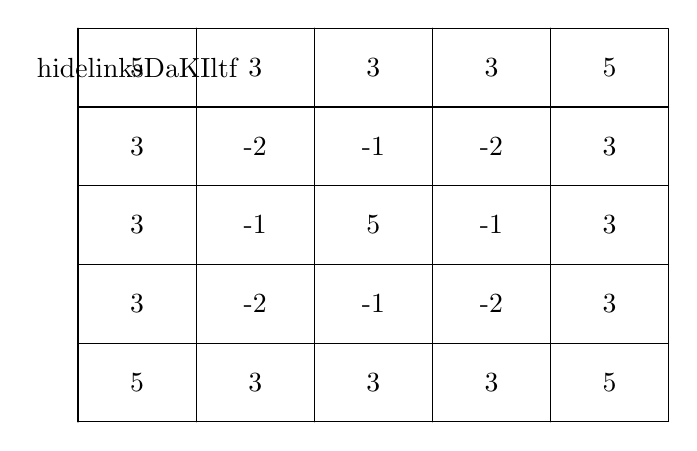
\begin{tikzpicture}[line join=round, line cap=round, >=stealth, scale=1]
			%điều chỉnh độ dãn rộng của bảng
			\def\r{1.5}
			\foreach \x [count=\i from 0] in {5,3,3,3,5}
			{\path (\r*\i,0) node{\x}; \global\let \n=\i}
			\foreach \x [count=\i from 0] in {3,-2,-1,-2,3}
			\path (\r*\i,-1) node{\x};
			\foreach \x [count=\i from 0] in {3,-1,5,-1,3}
			\path (\r*\i,-2) node{\x};
			\foreach \x [count=\i from 0] in {3,-2,-1,-2,3}
			\path (\r*\i,-3) node{\x};
			\foreach \x [count=\i from 0] in {5,3,3,3,5}
			\path (\r*\i,-4) node{\x};
			\foreach \y [count=\i from 0] in {0,1,2,...,4} {\draw ({\r*-0.5},-\i-0.5)--({\r*(\n+0.5)},-\i-0.5); \global\let \m=\i}
			\foreach \i in {0,1,...,\n} \draw ({\r*(\i-0.5)},0.5)--({\r*(\i-0.5)},-\m-0.5);
			\draw ({\r*-0.5},0.5) rectangle ({\r*(\n+0.5)},-\m-0.5);
			\path (0,0) node{\hypersetup{hidelinks}\href{DaKIltf}{ }};
		\end{tikzpicture}
	\end{center}
	Cách tính điểm như sau
	\begin{itemize}
		\item Ném ra ngoài bảng trừ $5$ điểm.
		\item Ném vào một trong $25$ ô điểm tính được ghi như trong bảng trên.
		\item Nếu sau $10$ lần ném mà\\
		- Đạt $50$ điểm thì nhận được phần quà trị giá $500\,000$ đồng.\\
		- Đạt từ $30$ điểm đến $49$ điểm thì nhận được phần quà trị giá $300\,000$ đồng.\\
		- Đạt từ $15$ điểm đến $29$ điểm thì nhận được phần quà trị giá $50\,000$ đồng.\\
		- Dưới $15$ điểm không có quà.
	\end{itemize}
	\begin{enumerate}
		\item Trong $9$ lần ném bi, bạn An ném được $5$ lần vào ô điểm $5$, một lần ra ngoài bảng, $2$ lần vào ô điểm $3$, một lần ô điểm $-1$. Tính số điểm bạn An nhận được sau $9$ lần ném.
		\item Hỏi bạn An có cơ hội nhận phần quà trị giá $300\,000$ không? Nếu có thì bạn An phải ném vào ô nào? Tính xác xuất để bạn An nhận được phần quà đó.
	\end{enumerate}
	\loigiai{
		\begin{enumerate}
			\item Tổng số điểm bạn An đạt được sau $9$ lần ném $5\cdot5-5+2\cdot3+(-1)=25$ điểm.
			\item Vì để nhận được phần quà trị giá $300\,000$ đồng bạn An phải đạt từ $30$ điểm đến $49$ điểm sau $10$ lần ném, mà $30-25=5$ điểm nên bạn An vẫn còn cơ hội để nhận quà.\\
			Do An đã ném $9$ lần nên để nhận quà bạn chỉ còn $1$ lần ném và phải ném vào ô điểm $5$.\\
			Có $5$ khả năng ném vào ô điểm $5$ trên tổng số $26$ khả năng (gồm $25$ ô trong bảng và $1$ khả năng ném ra ngoài).\\
			Nên xác suất để bạn An nhận phần quà trị giá $300\,000$ đồng là $\dfrac{5}{26}$.
		\end{enumerate}
	}
\end{bt}

\begin{bt}%[Dự án EX-9-Đề Cương Toán 9]%[Nguyễn Cường]%[9D6C2-2]
	Ở giữa mùa giải AFF CUP $2024 - 2025$, nơi mà những đội bóng hàng đầu Đông Nam Á tranh tài quyết liệt để giành lấy danh hiệu cao quý. Kết quả bảng B như sau
	\begin{center}
		\begin{tabular}{|c|c|c|c|c|}
			\hline
			Đội bóng & Số trận đấu & Số trận thắng & Số trận hoà & Số trận thua \\
			\hline
			Việt Nam & $4$ & $3$ & $1$ & $0$ \\
			\hline
			Philippines & $4$ & $2$ & $1$ & $1$ \\
			\hline
			Indonesia & $4$ & $1$ & $1$ & $2$ \\
			\hline
			Myanmar & 4 & 1 & 0 & 3 \\
			\hline
			Lào & 4 & 0 & 0 & 4 \\
			\hline
		\end{tabular}
	\end{center}
	Trong mỗi trận đấu, các đội sẽ được thưởng điểm như sau
	\begin{itemize}
		\item Một trận thắng là $3$ điểm.
		\item Một trận hoà là $1$ điểm.
		\item Một trận thua là $0$ điểm.
	\end{itemize}
	\begin{enumerate}
		\item Giả sử chọn ngẫu nhiên một đội bóng từ bảng B. Hãy tính xác suất chọn ra đội bóng có số trận thắng là $1$.
		\item Hãy tính xác suất để một đội bóng được chọn ngẫu nhiên có số điểm từ $4$ trở lên.
	\end{enumerate}
	\loigiai{
		\begin{enumerate}
			\item Do có $5$ đội bóng là Việt Nam, Philippines, Indonesia, Myanmar, Lào nên không gian mẫu của phép thử là $n(\Omega)=5$.\\
			Gọi $A$ là biến cố đội bóng có số trận thắng là $1$.\\
			Do chỉ có Indonesia và Myanmar có số trận thắng là $1$ nên $n(A)=2$.\\
			Xác suất để chọn ra một đội bóng có số trận thắng là $1$ là $\mathrm{P}(A)=\dfrac{n(A)}{n(\Omega)}=\dfrac{2}{5}=0{,}4$.
			\item Dựa vào kết quả bảng B, ta có số điểm của các đội như sau
			\begin{itemize}
				\item Việt Nam là $3\cdot3+1\cdot1+0\cdot0=10$.
				\item Philippines là $2\cdot3+1\cdot1+1\cdot0=7$.
				\item Indonesia là $1\cdot3+1\cdot1+2\cdot0=4$.
				\item Myanmar là $1\cdot3+0\cdot1+3\cdot0=3$.
				\item Lào là $0\cdot3+0\cdot1+4\cdot0=0$.
			\end{itemize}
			Gọi $B$ là biến cố đội bóng có số điểm từ $4$ trở lên. Do có $3$ đội bóng Việt Nam, Philippines, Indonesia có điểm thoả mãn nên $n(B)=3$.\\
			Xác suất để chọn ngẫu nhiên một đội bóng có số điểm từ $4$ trở lên là $\mathrm{P}(B)=\dfrac{n(B)}{n(\Omega)}=\dfrac{3}{5}=0{,}6$.
		\end{enumerate}
	}
\end{bt}
% In đáp án trắc nghiệm
\Closesolutionfile{ans}
\indapan{6}{ans/ans-9C8-OTC}

